\documentclass{report}


\usepackage{amsmath}

\usepackage{graphicx}

\usepackage{amsfonts}
\usepackage[]{algorithm2e}
\usepackage{booktabs}
\usepackage{floatflt}

\usepackage{pgfplots}

\begin{document}

\title{
\begin{figure}[htbp]
\centering

\includegraphics[scale=0.15]{logo.png}
\end{figure}
Artificial Intelligence\\
\begin{large} [1007315]
\end{large}}
\author{Jacopo Orlandini [286416]}


\maketitle

\begin{abstract}

Artificial intelligence (AI) has recently undergone a renaissance, making important progress in key areas such as control and decision making. This has been due, in part, to a large amount of available and cheap data and cheap compute resources, which have fit the natural strengths of deep
learning. In recent years, the quantity of information generated by business, government, and science has increase immensely - a phenomenon known as the \textit{data deluge}.
In parallel to this significant growth, data are also becoming increasingly interconnected. Facebook, for instance, is a graph nearly fully connected with 99.91 percent of individuals on the social network belonging to a single, large connected component.
Currently, most social networks connect people or groups who expose similar interests or features. More importantly, the interactions among people and exchange of huge amount of data have significantly developed new frontiers in data science.
In this project I dive into citation network. Citation network is a social network which contains paper resources and linked by co-citation relationship (also called citation graph).
Recent advancements in deep neural networks for graph-structured data have led to state-of-the-art performance on graph convolutional network and node embedding.
The representations learned using deep models can be used to enhance performance in a graph convolutional neural network, and these learned representations have high utility because they can be re-used in various tasks. For example, node embeddings can be used for citation recommendation. Deep learning methods have an increasingly critical role in recommender system applications, being used to learn useful low dimensional embeddings of text and individual users.
Recent years have seen significant developments in this space—
especially the development of new methods that are
capable of learning on graph-structured data, which is fundamental
for recommendation applications.

\end{abstract}


\chapter{Introduction}

\section{Artificial Intelligence}
\textit{In which we describe agents can improve their behaviour through diligent study of their own experiences.}
\vspace{0.3cm}

In artificial intelligence, an agent is an autonomous entity which observes through sensors and acts upon an environment using actuators and directs its activity towards achieving goals. Intelligent agents may also learn or use knowledge to achieve their goals \cite{agent}. An agent is learning if it improves its performance on future tasks after making observations about its environment. In our case the agent is a  artifact able to take a graph as input and producing inference pattern between nodes.
Learning has the advantage that it allows the agents to initially operate in unknown environments and to become more competent than its initial knowledge alone might allow. The most important distinction is between the \textit{learning element}, which is responsible for making improvements, and the \textit{ performance element}, which is responsible for selecting external actions.
A simple agent program can be defined mathematically as an function $f$ (called \textit{agent function}) which maps every possible percepts sequence to a possible action the agent can perform or to a coefficient, feedback element, function or constant that affects eventual actions.
\begin{equation}
f:P^* \rightarrow A
\end{equation}

There are three major types of learning:
In\textit{ unsupervised learning }the agent learn patterns in the input even though no explicit feedback is supplied. Clustering is the task of grouping a set of objects into groups based on the similarity of their features. Clustering belongs to exploration problems, where there is no knowledge about the state of the world. In \textit{reinforcement learning} the agent learns from a series of reinforcements-rewards or punishment. Reinforcement learning is an area of machine learning concerned with how software agents ought to take actions in an environment so as to maximize some notion of cumulative reward but requires clever exploration mechanisms. In \textit{supervised learning }, the agent observes some example input-output pairs and learns a function that maps input to output. In real world and real application, we can relax some constraints and create subset of these methods.
\section{Supervised Learning}
In semi-supervised learning we are given a few labeled examples and must make what we can of a large collection of unlabeled examples. Even the labels themselves may not be the oracular truths that we hope for. Thus, both noise and absence of labels create a continuum between supervised and unsupervised learning.
For semplicity I assume the task of supervised learning as milestone for semi-supervised: 
given a training set of N example input-output pairs
\[(x_1,y_1), (x_2,y_2),...(x_N,y_N)\] where $y_i$ was generated by an unknown relation $y_i = f(x_i),$ \\discover a function \[h\cong f\] that approximates \textit{f}.
To measure the accuracy of a hypothesis we give it a \textit{test set} of examples that are distinct from the training set. We say a hypothesis generalizes well if it correctly predicts the value of y for new examples. Sometimes the \textit{f} is stochastic, and we have to learn a conditional probability distribution.
When the output y is one of a finite set of values, we call the learning problem \textit{classification}. When y is a number, the learning problem is called \textit{regression}.

%\begin{figure}[htbp]
%\centering
%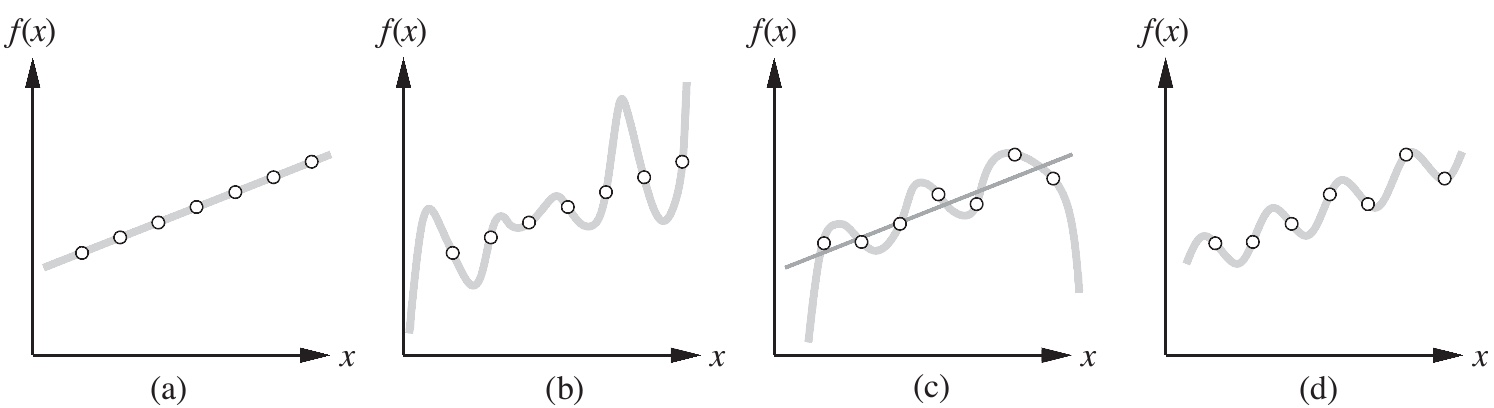
\includegraphics[scale=0.2]{function.jpg}
%\caption{(a) linear hypothesis. (b) degree-7 polynomial hypothesis for the same data. (c) regression (approximate linear fit). (d) sinusoidal fit to the same data set.
%\label{fig:mission}}
%\end{figure}

A classifier is a function that maps an unlabelled instance to a label using internal structures. The output is a set of expected labels for all instances in test set.
Estimating the accuracy of a classifier (agent function) induced by supervised (semi-supervised) learning algorithms is important not only to predict its future prediction accuracy, but also for choosing a classifier from a given set (model selection), or combining classifier (Wolpert 1992).
Based on available data, there are two possible philosophies,\textit{inductive learning} or \textit{transductive learning}.

Induction, in the context of learning, is the attempted discovery of patterns based on the analysis of collected data. The main characteristic of inductive learning is the building of a model – those rules/properties you induce from the data to answer your questions (statistical inference).

\subparagraph{Transductive} Transduction, in the context of learning, refers to reasoning from specific observed (training) instances, to specific observed (unlabelled) instances because we already use all possible instances. It is important to note that not all semi-supervised learning methods are transductive in nature. The main characteristic is the avoidance of building a general model. The information we learn cannot be used to label new instances (which did not have during training). Transductive learning is highly sensitive to noise samples. In my proejct since the embeddings are learned on the graph structure, the implemented method is transductive, which means we can only predict instances that are already observed in the graph at training time. However, it may be desiderable to have an inductive approach, where generalization hypothesis can be used to predict unseen instances.
%https://codesachin.wordpress.com/2016/07/03/a-small-and-easy-introduction-to-transductive-learning/

\subparagraph{Inductive biases}
Learning is the process of apprehending useful knowledge by observing and interacting with the
world. It involves searching a space of solutions for one expected to provide a better explanation
of the data or to achieve higher rewards. But in many cases, there are multiple solutions which
are equally good (Goodman, 1955). An inductive bias allows a learning algorithm to prioritize
one solution (or interpretation) over another, independent of the observed data (Mitchell,
1980). In a Bayesian model, inductive biases are typically expressed through the choice and
parameterization of the prior distribution (Griffiths et al., 2010). In other contexts, an inductive
bias might be a regularization term (McClelland, 1994) added to avoid overfitting, or it might
be encoded in the architecture of the algorithm itself. Inductive biases often trade flexibility
for improved sample% \usepackage{booktabs} complexity and can be understood in terms of the bias-variance tradeoff
(Geman et al., 1992). Ideally, inductive biases both improve the search for solutions without
substantially diminishing performance, as well as help find solutions which generalize in a
desirable way; however, mismatched inductive biases can also lead to suboptimal performance
by introducing constraints that are too strong.\cite{ind_BIAS}

\section{Graph Neural Network}
%https://arxiv.org/pdf/1806.01261.pdf
According to the explosion of social networks and Big Data, neural networks on graph have been developed and studied  for more than ten years under the umbrella of "graph neural network", but have grown rapdly in the last years.
Here we use \textit{graph} to mean a directed and weighted graph. In the common terminology, a graph is defined as a 2-tuple $G = ( V, A)$. The $V = \{v_i\}_{i=1:N^v}$ is the set of nodes (cardinality $N^v$), where each $v_i$ is a node attribute. The $E = \{(e_k,r_k,s_k)\}_{k=1:N^e}$ is the set of edges (of cardinality $N^e$), where each $e_k$ is the edge's attribute, $r_k$ is the index of the receiver node, and $s_k$ is the index of the sender node. We can easily extend the case of undirected or not-weighted graph.
In data science we can exploit graph properties via the spectral graph theory. The spectral graph theory studies the properties of graph via the eingenvalues and eigenvectors of their associated graph matrices: A (adjacency matrix) and graph Laplacian matrix).
One of the most difficult task for machine learning task is to develop appropriate representations for complex data like graph environment. 
In my project, I consider the problem of constructing a representation for data lying on a high-dimensional space (Bag-of-Words model)\footnote{Bag of Words: The bag-of-words model is a way of representing text data when modeling text with machine learning algorithms. Predominantly bag-of-words model is used in NLP (natural language processing) for document classification. BoW is a way of extracting features from text for use in modeling, but has different drawbacks. It suffers from some shortcomings, such as poor design of vocabulary, sparse representation of space.} and low-dimensional space (node embedding). Thanks to previous studies the graphs adapt well to the purpose of encoding structural information as protein structure\footnote{Protein structure prediction: is the inference of three-dimensional structure of a protein from its amino acid sequence. The aim of reasercher has been looking at the problem of protein structure matching}, social networks, citation networks and so on.
\subparagraph{Simple Graph}
A simple graph $\mathcal{G}=\{\mathcal{V}, \mathcal{E}\}$ is an undirected graph with neither multiple edges nor loops.
\begin{itemize}
\item $\mathcal{V}(\mathcal{G})= \{v_i,...,v_n\}$ is called the vertex set with n = $|\mathcal{V}|$
\item $\mathcal{E}(\mathcal{G})\subseteq \mathcal{V} \times \mathcal{V}$ is called the vertex set with m = $|\mathcal{E}|$
\item The number of neighbors of a node v is called the degree of v ($D$)
\item A graph is complete if there is an edge between every pair of
vertices.
\end{itemize}
A graph is called \textit{k-partite} if its set of vertices admits a partiotions into k classes such that the vertitces of the same class are not adjacent.
For simplicity I assume real-valued functions on the set of the graph’s
vertices, $f : V \Rightarrow R$. Such a function assigns a real number
to each graph node. In my project the function f restores a list of features for each node.

\subparagraph{Adjacency Matrix} For a graph with n vertices, the adjacency matrix is defined by $n \times n$ and:
\begin{equation}
A := \begin{cases}
A_{ij} = 1 & \text{if there is an edge $e_{ij}$}\\
A_{ij} = 0 & \text{if there is not an edge}\\
A_{ii} = 0 
\end{cases}
\end{equation}
A is a real-symmetric matrix with n real eingenvalues and its n real eigenvectors form an orthonormal basis.
The adjacency matrix can be viewed as an operator:
\begin{equation}
 g = Af;\ g(i) = \sum_{e_{ij}} f(j) 
 \end{equation}
It can be viewed also as a quadratic form:
$f^T A f =  \sum_{e_{ij}} f(i)f(j) $\\
The connection between the Laplacian and the adjacency matrices:
 $L = D - A$

\subparagraph{Laplacian Matrix}
In the mathematical field of graph theory, the Laplacian matrix, sometimes called admittance matrix, Kirchhoff matrix or discrete Laplacian, is a matrix representation of a graph. The Laplacian matrix can be used to find many useful properties of a graph.

Given a simple graph G with n vertices, its Laplacian matrix $L_{n\times n} $ is defined as: $ L = D-A$ 
where D is the degree matrix and A is the adjacency matrix of the graph. Since \textit{G} is a simple graph, \textit{A} only contains 1s or 0s and its diagonal elements are all 0s.

In the case of directed graphs, either the indegree or outdegree might be used, depending on the application.

The elements of $L$ are given by:
\begin{equation}
L_{i,j}= 
\begin{cases}
deg(v_i) & \text{if $i=j$}\\
-1 &	\text{if $i \neq j$ and $v_i$ is adjacent to $v_j$}\\
0 &\text{otherwise}\\
\end{cases}
\end{equation}

The symmetric normalized Laplacian matrix is defined as:
\begin{equation}
L^{sym} = D^{-\tfrac{1}{2}} L D^{-\tfrac{1}{2}} = I -D^{-\tfrac{1}{2}} A D^{-\tfrac{1}{2}} 
\end{equation}

The elements $L^{sym}$ are given by:
\begin{equation}
L^{sym}_{i,j}= 
\begin{cases}
1 & \text{if $i=j$ and deg$(v_i) \neq 0$}\\
-\tfrac{1}{\sqrt{deg(v_i)deg(v_j)}} &\text{if $i \neq j$ and $v_i$ is adjacent to $v_j$}\\
0 &\text{otherwise}\\
\end{cases}
\end{equation}

%fa cagare l'immagine
The Laplacian allows to link between discrete representations (e.g graph, linked structures) and continuous representation (e.g vector space)\footnote{For example we can map a graph on a line such that connected nodes stay as close as possible (i.e arg min$(f^T L f )$ with $f^Tf=1$)}.
We can see Laplacian as an operator in simple graph weighted as:
\begin{equation}
f^T L f = \dfrac{1}{2}\sum_{e_{ij}} w_{ij}|f(v_i)-f(v_j)|^2    \text{            	with $w_{ij}>0$} 
\end{equation} 


\subparagraph{Graph Partitioning Problem}
The main application of laplacian is spectral clustering that corresponds to a computationally performant solution to the graph partitionning problem \\
Given: 
$G = (V, E) $ and  P number of partitions.\\ Output:
	Compute a (vertex) partition $V=V_0 \cup V_1 \cup ... V_{p-1}$ such that:
	\begin{enumerate}
	\item $ \{V_i \} $ are disjoint $\Rightarrow V_i \cap V_j = \oslash$
	\item $ \{V_i \} $ are roughly balanced $\Rightarrow |V_i| \approx |V_j| $
	\item let $E_{cut} \equiv \{ (u,v) | u \in V_i, v \in V_j, i \neq j\} $ :  minimize $E_{cut}$
	\end{enumerate}

\begin{figure}[htbp]
\centering
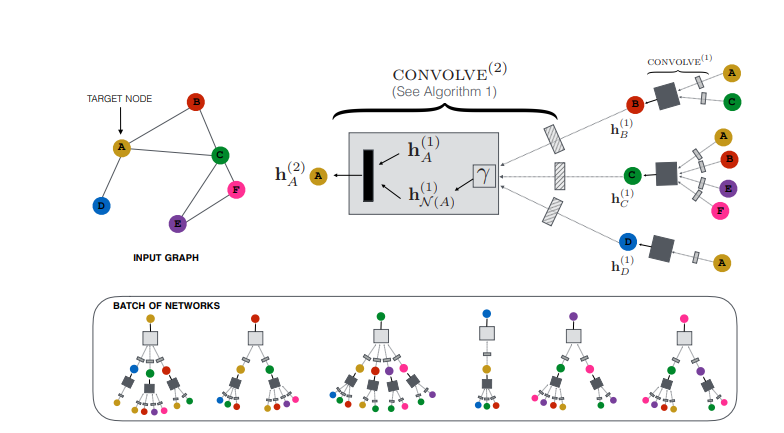
\includegraphics[scale=0.3]{gconv.png}
\caption{Graph using depth-2 convolution}
\label{fig:conv}
\end{figure}

\subsection{Learning Architectures}
%https://arxiv.org/pdf/1806.01973.pdf
Most prominent among these advancements is the success
of deep learning architectures known as Graph Convolutional
Networks (GCNs). The core idea behind GCNs is
to learn how to iteratively aggregate feature information from local
graph neighborhoods using neural networks. In figure \ref{fig:conv} I show a 
single “convolution” operation transforms and aggregates feature
information from a node’s one-hop graph neighborhood, and by
stacking multiple such convolutions information can be propagated
across far reaches of a graph. Unlike purely content-based deep
models (e.g., recurrent neural networks), GCNs leverage both
content information as well as graph structure. 
The main challenge is to correctly size and find the right combination of both the BoW as well as node embeddings.\cite{deep_GCN}.





\section{Related Work}
In this project we consider the problem of classifying nodes (such as scientific documents) in a directed graph,  where the labels are only available for a small subset of nodes. This problem can be framed as graph-based semi-supervised learning. \cite{Kipf_GCN}. Given a network of citations and a reduced amount of labels, the agent try to predict node label from its knowledge base.


\section{State of the Art}
In this section I present the state of the art regarding the main technologies used in the project.
First of all I contextualize on neural networks.
\subsection{Object Classification Problem}
In this problem we have a set of objects, which can be document and we may suppose that the numerical representation of an object is a n-dimensional vector $x \in R^n$. There exists a function $f : R^n \rightarrow \{1, 2, . . . , K\}$, that associate to each object x a class $f(x)$, where $K \in \mathbb{N}$ (also known as label), is the number of different classes (e.g. x is an image and f(x)
is the class \textit{dog}). The solution to the classification problem consists in
determining a function equivalent to $f$ (also known as hypothesis).
The classification problem can also be related to other tasks such as node detection in graph.

The output of the NN, is a highly complex non-linear function $z(x) \in \mathbb{R}^K$,
which, in turn, is dependent on the (trainable or not) parameters of the NN. This function is used to obtain a probability distribution of the class $j$ given the object $x$, called the
\textit{softmax function}. If $z_j(x)$ is the j-th component of $z(x)$, with  j = 1, . . . , K then the \textit{softmax} function is given by:
\begin{equation}
\sigma_j(z) = P(y=j | x) = \dfrac{e^{z_j(x)}}{\sum_{i=1}^{K} e^{z_i(x)}}
\end{equation}

\subparagraph{Softmax Function}For example, given a 7-dimensional vector $(1;2;3;4;1;2;3)$ the softmax function produce $(0.024;\ .064;\ .175;\ .475;\ ...)$.\\
In mathematics, the softmax function, also known as \textit{softargmax}, is a function that takes as input a vector of $K$ real numbers, and normalizes it into a probability distribution consisting of $K$ probabilities. After applying softmax, each component will be in the interval $(0,1)$ and the components will add up to $1$. \textit{Softmax} is used in NN to map the non-normalized output of a network to a probability distribution over predicated output classes.



The goal is to obtain a softmax function such that $f(x)=argmax_jp(j|x)$.
In order to do this a NN is trained using a training set T. Each element of T is a couple $(x_i,f(x_i)), i=1,2,...,N$ and N is the size of the training set. In order to determine the accuracy of the network, a loss function is employed, that assigns to each object x a quantitative measure of the error the NN made in
classifying x. Often, the loss function takes the negative logarithm of the softmax function as follows
\[
L(x)=-log\ p(f(x)|x)
\]
and, in order to improve the NN, the gradients (with respect to the parameters of the NN, hidden in the definition of z) of the mean of the loss function over all training set
\[
L = -\dfrac{1}{N}\sum_{i=1}^{N} log\ p(f(x_i)|x_i) 
\]
are back propagated along all the layers of the NN. The negative logarithm of the softmax function can be interpreted as the \textit{cross-entropy} between the probability
distribution given in softmax function and the true probability $q(j|x)$ of the class $j$ given the object $x$.

\[
\mathbb{H}(q,p) = - \sum_{i=1}^{K} q(i|x) log\ p(i|x) 
\]
In most of the literature regarding the cross-entropy loss function in NN, the
probability distribution q is taken as follows
\begin{equation}
q(j|x)= 
\begin{cases}
1 & \text{if $f(x)=j$ }\\
0 &\text{otherwise}\\
\end{cases}
\end{equation}
and having chose q as above, and substituting it in $\mathbb{H}$, one obtains \\ $L(x)=-log\ p(f(x)|x)$  which
is commonly referred to as the categorical cross-entropy. One of the main problem in training a neural network is the over-fitting. The
over-fitting of a neural network, is the problem that prevent the network to generalize
and obtain accurate prediction on samples not contained in the training set. Moreover and worse, one finds that, sometimes, the training process spends a
lot of time to reduce the loss without even achieve better fitting on the training
set. With a close inspection in fact one can observe that a considerable amount
of the time is spent, by the training process, on Loss function to make better an already good and accurate prediction.

\subsection{Graph Convolutional Neural Networks}
%https://towardsdatascience.com/how-to-do-deep-learning-on-graphs-with-graph-convolutional-networks-7d2250723780
%https://tkipf.github.io/graph-convolutional-networks/
Today, graph convolutional neural networks are a powerful neural network architecture for machine learning on graphs. In fact, they are so powerful that even a randomly initiated 2-layer GCN can produce useful feature representations of nodes in networks. For these models, the goal is to learn a function of signals/features on a graph, a GCN takes as input:
\begin{itemize}
\item an input feature matrix $N \times F^0$, feature matrix $X$, where N is the number of nodes and $F^0$ is the number of input features for each node (BoW has 1433 features + optional node embedding).
\item an $N \times N$ matrix representation of the graph structure such as the adjacency matrix A of $\mathcal{G}$.
\end{itemize}
and produces a node-level output $Z$ (an $N \times F$ feature matrix where $F$ is the number of output features per node). 

A hidden layer in the GCN can thus be written as $H^i = f(H^{i-1},A)$ where $H^0 = X$ and $f$ is the propagation function. Each layer $H^i$ corresponds to an $N \times F^i$ feature matrix where each row is a feature representation of a node. At each layer, these features are aggregated to form the next layer’s features using the propagation rule \textit{f}. Graph-level output can be modeled by introducing some form of pooling operation that do not introduce any trainable parameters.
In this way, features become increasingly more abstract at each consecutive layer. In this framework, variants of GCN differ only  L being the number of layers. 
%https://arxiv.org/pdf/1806.01973.pdf
To recap $H^{(0)} = X$ and $H^{(L)}= Z $. The specific models then differ only in how $f(\_ \ , \_)$ is chosen and parameterized.
In \cite{Kipf_GCN} they arrive at the propagation rule:
\[
f(H^{(l)}, A) = \sigma (\hat{D}^{-\tfrac{1}{2}} \hat{A} \hat{D}^{-\tfrac{1}{2}} H^{(l)}W^{(l)}) 
\]
with: 
\begin{itemize}
\item $\hat{A}= A +I$ (adjacency matrix)
\item $\hat{D}$ is the diagonal node degree matrix of $\hat{A}$.
\item $\sigma$ is a non-linear activation function like the ReLU
\item $W^{(l)}$ is a weight matrix for the l-th neural network layer.
\end{itemize}

\subsection{Semi-supervised Node Classification}
%https://arxiv.org/pdf/1609.02907.pdf
%https://arxiv.org/pdf/1603.08861.pdf
As outlined in the introduction,
we can relax certain assumptions typically made in graph-based semi-supervised learning
by conditioning our model f(X, A) both on the data X and on the adjacency matrix A of the
underlying graph structure. We expect this setting to be especially powerful in scenarios where the
adjacency matrix contains information not present in the data X, such as citation links between documents
in a citation network or relations in a knowledge graph. The overall model is 2 layer GCN.Their forward model then takes the simple form:
\[
Z = f(X,A) = softmax(\hat{A}\ ReLU(\ \hat{A}XW^{(0)}\ )W^{(1)})\ .
\]

\subsection{Node Embedding node2vec}
Prediction tasks over nodes and edges in networks require careful
effort in engineering features used by learning algorithms. Recent
research in the broader field of representation learning has led to
significant progress in automating prediction by learning the features
themselves. In \cite{n2v} Node2vec, an algorithmic framework for learning
continuous feature representations for nodes in networks. In
node2vec, we learn a mapping of nodes to a low-dimensional space
of features that maximizes the likelihood of preserving network
neighborhoods of nodes.
\paragraph{Feature learning framework}
Let $f: V \rightarrow \mathcal{R}^d$ be the mapping function from nodes to feature representations we aim to learn for prediction task. here $d$ is a parameter specifying the number of dimension of our feature representation. $f$ is a matrix of size $|V| \times d$ parameters. For every source node $u \in V$, we define $N_S(u) \subset V$ as a network neighborhood of node $u$ generated through sampling strategies. In node2vec we seek to optimize the following objective function:
\[
\max_{f} \sum_{u \in V} log\ Pr(N_S(u)|f(u)).
\]
In order to make the optimitation problem tractable there are two main assumptions:
\begin{itemize}
\item Conditional indipendece of neighborhood
\[
Pr(N_S(u)|f(u) =  \prod_{n_i \in N_S(u)} Pr(n_i|f(u). 
\]
\item Symmetry in feature space: softmax unit parametrized by a dot product of their features.
\[
 Pr(n_i|f(u) = \dfrac{exp((fn_i) \cdot f(u))}{\sum_{v \in V} exp(f(v) \cdot f(u))}
\]

\end{itemize}
 
In this project, I use node2vec framework to build a low dimensional space of features that maximize the likelihood of preserving network neighborhoods of nodes. In typical node classification task, we are interested in predicting the most probable labels of nodes in a network. In link prediction, we wish to predict whether a pair of nodes in a network should have an edge connecting them. The problem of sampling neighborhoods of a source has a critical role for create embedding features. Generally there are two strategies for generating neighborhood set of nodes: Breadth-First Sampling (BTS) and Depth-first Sampling (DFS). 
Node2Vec designs a flexible neighborhood sampling strategies which allows us to smoothly interpolate between BFS and DFS.
\paragraph{Random Walks}
Formally given a source node $u$, this framework simulate a random walk of fixed lenght $l$. Let $c_i$ ($i$th node in the walk), starting with $c_0=u$ (source node). Nodes $c_i$ are generated by the following distribution:
\[
P(c_i = x | c_{i-1} = v) =  
\begin{cases}
\dfrac{\pi_{vx}}{Z} & \text{if $(v,c) \in E$ }\\
0 &\text{otherwise}\\
\end{cases}
\]
where $\pi_{vx}$ is the unnormalized transition probability between nodes v and x, and $Z$ is the normalizing constant.
\paragraph{Search Bias $\alpha$}
The simplest way to bias our random walks would be to sample
the next node based on the static edge weights $w_{vx}$ i.e., $π_{vx}$ = $w_vx$.
(In case of unweighted graphs $w_{vx} = 1$.) However, this does not allow us to account for the network structure and guide our search procedure to explore different types of network neighborhoods.

 We set the unnormalized
transition probability to $\pi_{vx} = \alpha_{pq}(t, x) · w_{vx}$, where:
\[
\alpha_{pq}(t, x) =  
\begin{cases}
\dfrac{1}{p} & \text{if $d_{tx} = 0$ }\\
1 & \text{if $d_{tx} = 1$ }\\
\dfrac{1}{q} & \text{if $d_{tx} = 2$ }\\
\end{cases}
\]
where $d_tx$ denotes the shortest path distance between nodes t and x.
For semplicity, we assume that parameters p and q control how fast the walk explores and leaves the neighborhood of starting node $u$.
\\Parameter p controls the likelihood of immediately
revisiting a node in the walk. 
\begin{itemize}


\item Setting it to a high value
$(> max(q, 1))$ ensures that we are less likely to sample an alreadyvisited
node. 
\item Therefore if p is low $(< min(q, 1))$, it would lead the walk to
backtrack a step and this would keep the walk “local”
close to the starting node u.
\end{itemize}

Parameter q allows the search to differentiate between “inward” and “outward” nodes.
\begin{itemize}

\item  if $q > 1$, the random walk is biased towards nodes close to node t.
\item  In contrast, if $q < 1$, the walk is more inclined to visit nodes
which are further away from the node t.
\end{itemize}
For current subsection I refer to \cite{n2v}

\section{Methods}
Here we present the problem setup over the \cite{Kipf_GCN} architecture.

\subsection{Loading Data}
\subsection{Features Retrieval}
In the architecture provided, we can ascertain the presence of the $X$, matrix representation of BoW model, and $A$, matrix representation of the adjacency graph. 

Moreover we introduce the \textit{embedding nodes matrix} that is
jointly trained with $X$ to predict the class label of the instance and therefore the context in the graph. We concatenate the embeddings
and the X of the original classifier and feed them to a softmax layer when making the prediction.
\subparagraph{Concatenation operation}
\[
conc (
\begin{bmatrix}
    x_{1,1}       & x_{1,2} & \dots & x_{1 ,n} \\
    x_{2,1}       & x_{2,2} & \dots & x_{2 ,n} \\
    \vdots  & \vdots & \ddots & \vdots \\
    x_{d,1}       & x_{d,2} & \dots &x_{d ,n} \\
\end{bmatrix}
\begin{bmatrix}
    e_{1,1}       & e_{1,2} & e_{1,3} & e_{1,4}\\
    e_{2,1}       & e_{2,2} & e_{2,3} & e_{2,4}\\
    \vdots  & \vdots & \ddots & \vdots \\
    e_{d,1}    & e_{d,2} & \dots &x_{d ,4} \\
\end{bmatrix}
)
=
\begin{bmatrix}
    x_{11} & x_{12} & x_{13} & \dots  & e_{1,n+4} \\
    x_{21} & x_{22} & x_{23} & \dots  & e_{2,n+4} \\
    \vdots & \vdots & \vdots & \ddots & \vdots \\
    x_{d1} & x_{d2} & x_{d3} & \dots  & e_{d,n+4}
\end{bmatrix}
\]
This way of creating a matrix is called horizontal concatenation. For example, concatenate two row vectors of a matrix to make an even longer row vector. To concatenate two matrices $hconc(X,E)$, they must have compatible sizes in rows.
\paragraph{Grid Search}
In machine learning, hyperparameter optimization or tuning is the problem of choosing a set of optimal hyperparameters for a learning algorithm. A hyperparameter is a parameter whose value is used to control the learning process. By contrast, the values of other parameters (typically node weights) are learned.
As regards the search for the optimal node2vec parameters, we have used the grid search strategy.
\paragraph{k-fold cross validation}
As first test we use cross-validation to assessing the trained model but with some limitations. First of all we can not guarantee that all the classes in the citation network are present in the training set. Then we randomly choose instances of test set without balancing. 
In a second approach, we have studied (custom) cross validation in such a way that the current slice is accepted only if the number of classes per type exceeds a certain treshold. The treshold is set to be 14.2\% of the size of the training set (empirical method for calculating treshold
 ).
\[
treshold = \lfloor \dfrac{2708*0.052}{(7*2) + 1} \rfloor = 9 
\]
%https://www.researchgate.net/profile/Ron_Kohavi/publication/2352264_A_Study_of_Cross-%Validation_and_Bootstrap_for_Accuracy_Estimation_and_Model_Selection/links/02e7e51bcc14c5e91c000000.pdf


\section{Experiments and Results}

\subsection{Dataset}
We test this new framework on the following dataset:
\paragraph{Cora} In the Cora dataset, nodes represent document, and edges represet citation between them. The citation network has  2708 and 5249 edges. The dataset contain sparse bag-of-words feature vector for each document and a list a list of citation links between documents. Each document has a class label (total 7  classes). 
\begin{table}[htb]
\centering

\begin{tabular}{|c|c|c|c|c|c|}
\toprule
Dataset & Nodes & Edges & Classes & Features & Label Rate \\ \midrule
Cora    &  2708   & 5429    &  7   &  1433 & 0.052   \\
\end{tabular}
\end{table}

\subsection{Experimental Set-Up}
For this project we use this simple configuration:
At the beginning of every run of \textit{custom} cross validation we shuffle the entire dataset, keeping the correspondences w.r.t the initial loaded data (X, A).
We import the optimal node embedding model and consequently normalize that matrix and add to X to create the final features matrix. We use

\begin{itemize}

\item \textbf{training set} equals to $t=size(Cora,5.2\%)$ of dataset.
\item \textbf{validation set} equals to $\dfrac{size(Cora,100\%) - t}{2}$ of dataset.
\item \textbf{test set} equals to remain nodes of dataset.
\end{itemize}
In the custom cross-validation we set 10\% of t as treshold to accept the minimum number of classes in the training set k-fold.
At every k-fold we reinitialize weights and biases and let's move forward in the next slice. For moving in the next slice we use a simple but effective way. 

\paragraph{Custom Cross Validation} For this task, I create a support vector $\mathcal{S}$ with shuffled Y indices as elements.\\
For example we assume that Y is an incremental series from 0 to N.
\[
 \mathcal{S} =
 \begin{bmatrix}
           s_{1} \\        
           \vdots \\
           s_{t}\\
			\vdots \\
           s_{N}
         \end{bmatrix}= 
          \begin{bmatrix}
           y_{1} \\        
           \vdots \\
           y_{t}\\
			\vdots \\
           y_{N}         \end{bmatrix}=
                     \begin{bmatrix}
           2 \\        
           \vdots \\
           144\\
			\vdots \\
           456         \end{bmatrix}
\]

For the task of moving to the new slice, we simply remove t (as define above in size\_fold) elements in head and append to tail of . The result is 
For the task of moving to the new slice, we simply remove t (as define above) elements in head and append to tail of . The result is 
\[
\mathcal{S} =
 \begin{bmatrix}
           s_{t+1} \\        
           \vdots \\
           s_{N}\\
           s_{1}\\
			\vdots \\		
           s_{t}
           \end{bmatrix}
\]
and so on. Thanks to $\mathcal{S}$ we can get indices to retrive the one-hot encode on Y (label). Remember that we must keep consistency between X, A and model set like training set and so on.
To increase statistical accuracy we repeat training and prediction tasks 5 times over the current fold, then we return the average. 
\paragraph{Normalization}
We use normalization just for node embedding matrix.
In this project are implemented:
\begin{itemize}
\item Feature Scaling: is a method used to standardize the range of independent variables or features of data. In data processing, it is also known as data normalization and is generally performed during the data preprocessing step.
\[
x' = \dfrac{x - min(x)}{max(x)-min(x)}
\]
\item Standarditation:
In statistics, the standard score is the signed fractional number of standard deviations by which the value of an observation or data point is above the mean value of what is being observed or measured. Observed values above the mean have positive standard scores, while values below the mean have negative standard scores.
\[
z = \dfrac{x- \mu }{\delta}
\]
where $\mu$ is the mean and $\delta$ is the standard deviation.
\end{itemize}
In this project I normalize each column, instead of row.

\subsection{Results}
First of all we present the current custom cross validation accuracy on the same architecture of \cite{Kipf_GCN}.
\paragraph{Standard Cross Validation} High-level parameters are:
\begin{itemize}
\item Total Run: 100
\item EPOCH total: 200
\item inner loop on fold: 5
\item PATIENCE: 10
\item FILTER: localpool
\item label rate: 0.052
\item Dataset: Cora
\end{itemize}
The final accuracy is the average of all 100 runs:  0.7551.
\paragraph{Node Embedding}
We compute both undirected graph node embedding and directed.
Note that Cora is a citation network with directed graph.
The optimal solution with Feature Rescaling normalization is:\\\\
\begin{table}[htb]
\centering

\begin{tabular}{|c|c|c|c|c|c|}
\hline
Dimension & LenWalk & NumWalk & P & Q& Accuracy \\ 
\hline
4    &  10   & 100  &  0.1   &  2 & 0.809   \\
\hline
\end{tabular}
\end{table}

Below we present the 3d representaion of the architecure and its accuracy in relation to parameters :

\begin{figure}[htbp]
\centering
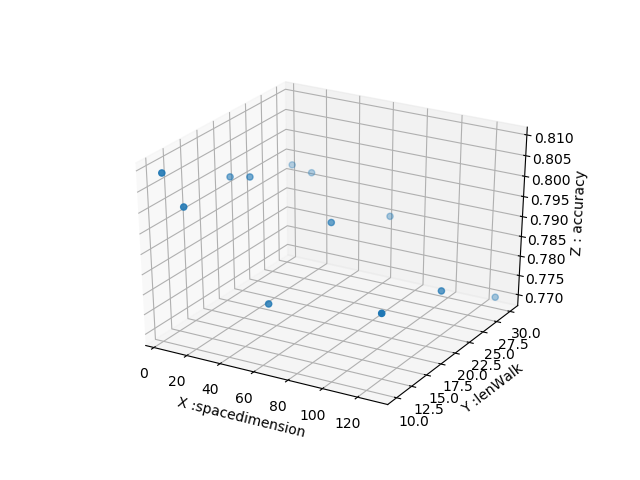
\includegraphics[scale=0.7]{01.png}
\caption{Graph using spaceDim and LenWalk}
\label{fig:01}
\end{figure}

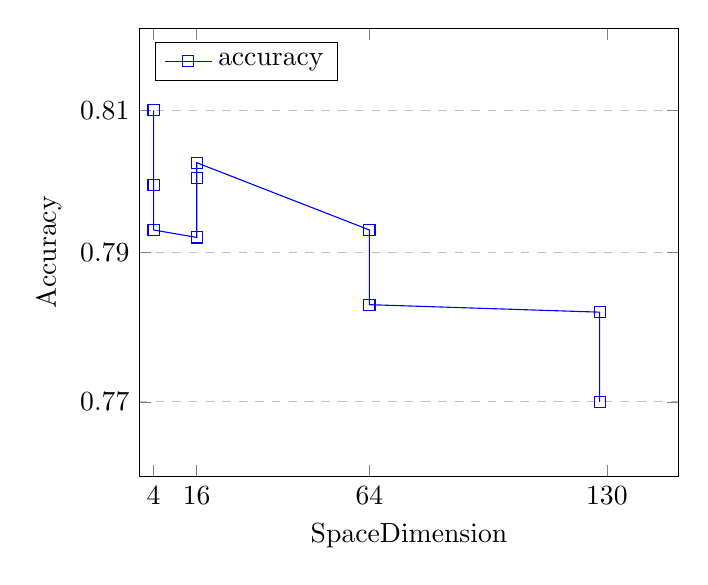
\begin{tikzpicture}
\begin{axis}[
    xlabel={SpaceDimension},
    ylabel={Accuracy},
    xmin=0, xmax=150,
    ymin=0.76, ymax=0.82,
    xtick={4, 16, 64,130},
    ytick={0.77, 0.79, 0.809},
    legend pos=north west,
    ymajorgrids=true,
    grid style=dashed,
]
 
\addplot[
    color=blue,
    mark=square,
    ]
    coordinates {
    ( 4.0 , 0.809 ) ( 4.0 , 0.799 ) ( 4.0 , 0.793 )
	( 16.0 , 0.792 ) ( 16.0 , 0.8 )( 16.0 , 0.802 ) 
    ( 64.0 , 0.793 ) ( 64.0 , 0.783 )
    ( 128.0 , 0.782 )( 128.0 , 0.77 )  };
    \legend{accuracy}
\end{axis}
\end{tikzpicture}
 
%  y = -1.651954603·10-4 x + 8.027553594·10-1
\begin{figure}[htbp]
\centering
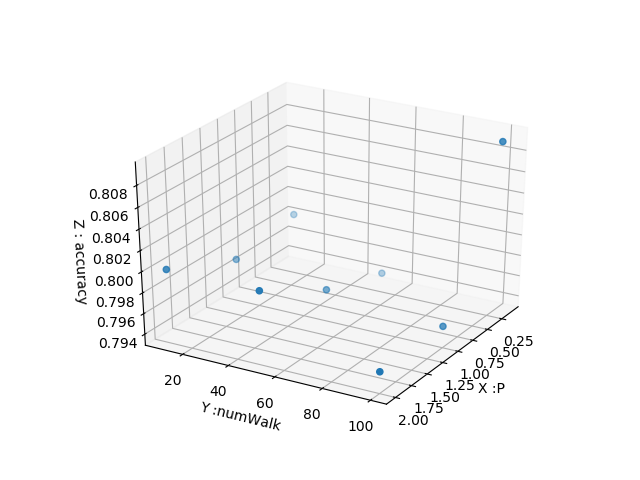
\includegraphics[scale=0.7]{23.png}
\caption{Graph using NumWalk and P}
\label{fig:23}
\end{figure}

\section{Conclusion}
The composition between the bag of word model and the node embedding model has led to a performance increase of about 5 percentage points.
Working mainly on a pre-existing architecture, introduced by Kipf, Thomas N and Welling, Max, the task was to adjust the parameters of the node embedding and create a custom cross-validation for our dataset.
This result gives us the best tuning hyperparameter for node2vec: In order to discover which nodes have the same structural structure roles we use q = 2 and p = 0.1. The random walk so is biased towards neighboring nodes (BFS).
In particular, it is noted that the accuracy decreases with respect to the increase in the size of the space associated with node2vec. I suspect that the best configuration for dimSpace is equal to the number of classes in the choosen dataset. 
Going to concatenate the bag of word model matrix with 1433 characteristics with node2vec, we notice a graceful decay in the increase in the ratio between the number of features used in Bow and that of node2vec. So we probably need to minimize the number of features in node2vec.
Regarding the \textit{numWalk} of the path of the random walk, we realize that the maximum accuracy is reached when the size is close to the label rate used in the training set.
In the approach used it was reasonable that the maximum path (\textit{lenWalk}) length is minimal. In fact, the maximum accuracy is obtained for short paths that optimally describe the structure of the neighbors of the node.\\

In my test the final accuracy for the embedding case on 100 runs is : 0.8046950515176832 with node2vec parameters as:
\begin{itemize}
\item spaceDim = 4
\item lenWalk = 10
\item numWalk = 100
\item P = 0.1
\item Q = 2
\end{itemize}


\begin{table}[htb]
\caption{Results}


\begin{tabular}{|c|c|c|c|c|c|c|c|}
\toprule
Dataset &Embedding & E-Normalization & E-Edges & Accuracy & cCV & Treshold & Total Run\\ \midrule
Cora    &no&  -   & - &  0.7551  & yes  & no & 100\\
%Cora    &yes&  MinMax   & undirected &  0.806  & NO  & no & 1\\
%Cora    &yes&  MinMax   & directed &  0.809  & NO   & no & 1\\
%Cora    &yes&  Std   & directed &  0.804  & NO  & no & 1 \\
Cora    &no	&  -   & - &  0.8043  & yes  & 9 & 100 \\
Cora    &yes&  MinMax   & directed &  0.8046  & yes  & 9 & 100\\
\hline
\multicolumn{5}{l}{cCV: custom cross validation, E: embedding}
\end{tabular}
\end{table}
\begin{figure}[htbp]
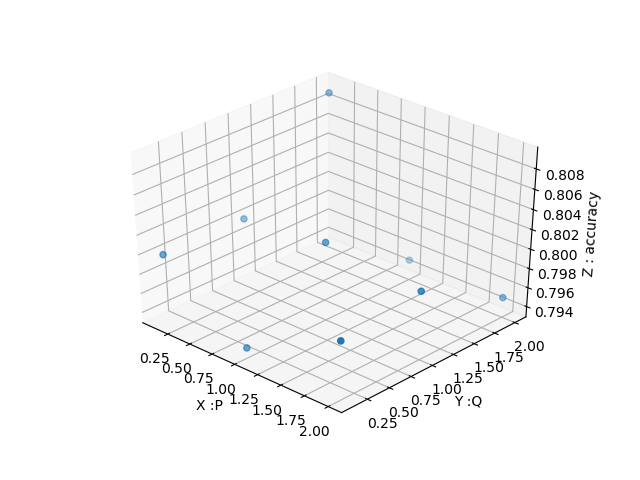
\includegraphics[scale=0.7]{34.png}
\caption{Graph using P and Q}
\label{fig:34}
\end{figure}

\bibliographystyle{plain}

\bibliography{example1}

\end{document}
